\documentclass[preprint,12pt]{elsarticle}
\usepackage[UTF8,fontset=windows]{ctex}
\usepackage{graphicx}
\usepackage{float}
\usepackage{xurl}
\usepackage{needspace}
\usepackage{amsmath,amssymb}
\usepackage{booktabs,tabularx,array}
\usepackage{enumitem}
\biboptions{numbers,sort&compress}
\usepackage{xcolor,tikz}
\usetikzlibrary{positioning,arrows.meta}
\usepackage[colorlinks=true,linkcolor=blue!45!black,citecolor=blue!45!black,urlcolor=blue!45!black,breaklinks=true]{hyperref}
\setlength{\emergencystretch}{2em}
\setlist{nosep,leftmargin=*}
\newcolumntype{Y}{>{\raggedright\arraybackslash}X}
\journal{Journal of Parallel and Distributed Computing}
\makeatletter
\let\ps@pprintTitle\ps@plain
\makeatother
\begin{document}
\begin{frontmatter}
\title{面向状态变化的诊断技能复用：\\SGLang PD 分离推理的 Agent 自动调优}
\author{BoTao Cheng}
\address{Tencent}
\date{}


\begin{abstract}
预填充与解码（PD）分离使大语言模型服务能够分别配置阶段资源、并行策略、批处理与状态传输。本文在昆仑芯 P800 资源池上开展 SGLang 部署实验，观察到缓存复用、重启流程及空闲恢复会改变名义相似配置的执行表现；总吞吐增加时，单卡效率或 token 生成时延也可能恶化。针对这些问题，本文提出基于历史经验约束的诊断技能与 Agent 自动调优框架。技能描述适用状态、有边界的干预、竞争解释、预期观测、恢复流程及支持证据；语言模型控制器选择诊断动作与参数族，受约束数值优化器提出具体配置。能力与执行契约限定允许的操作，上下文变化触发适用性检查，并在必要时重放诊断。框架分别记录诊断支持、进程存活、请求完成与服务目标达标。部署实验为设计提供动机，评价方法通过数值搜索、固定规则与 Agent 技能选择的同条件比较，检验各组件的作用。本文关注在可修正错误经验的前提下，降低找到可行服务配置的完整调优成本。

\end{abstract}

\begin{keyword}
大语言模型推理服务\sep 预填充与解码分离\sep Agent 自动调优\sep 诊断技能\sep 资源规划
\end{keyword}
\end{frontmatter}

\section{引言}
大语言模型推理配置涉及资源分配、并行执行、批处理、内存管理和通信。预填充与解码分离（prefill--decode disaggregation，以下简称 PD 分离）将提示词处理与后续 token 生成分配到不同阶段，在支持阶段专属配置的同时引入显式状态传输。DistServe 研究时延约束下的资源分配，Splitwise 探索分阶段硬件配置，HexGen-2 联合考虑异构资源与通信\cite{distserve2024,splitwise2024,hexgen2025}。高效服务因此需要协调推理阶段及其连接关系。

在评价下一组配置之前，调优器首先需要决定获取什么证据。时延上升可能来自预填充压力、解码准入、缓存加载或状态传输等待，不同解释对应不同干预方向。搜索全部参数族可能消耗大量部署预算；未经检验就采纳某个看似合理的解释，又可能将错误经验传播到后续任务。

本文在 P800 上开展 SGLang 预实验，观察到缓存复用与执行协议对吞吐和时延有明显影响。在一次配置比较中，增加预填充资源提高了总吞吐，却降低了单卡吞吐；另一些运行没有进程崩溃，但仅完成少量请求。持续满压与长时间空闲后的恢复测试也暴露出不同故障路径。这些现象促使本文在复用调优经验之前显式检查执行状态。

大语言模型辅助调优已有领域知识、数值优化与经验积累等研究。GPTuner 将调优知识用于优化，STELLAR 积累上下文规则，SysInsight 将系统内部机制与实测诊断联系起来\cite{gptuner2024,stellar2025,sysinsight2026}。本文进一步聚焦诊断动作：什么受控观测能够区分竞争性的阶段解释，以及诊断建议在什么条件下可以复用。

本文提出经验约束诊断技能框架，由语言模型控制器、人工编写的技能库、数值优化器，以及独立执行器与评价器组成。技能显式声明适用条件、允许的干预、预期观测和恢复流程。历史经验用于调整搜索优先级；缓存状态、软件、拓扑或初始化条件变化后，控制器重新检查适用性，必要时重放诊断，避免永久排除其他合法配置。

本文包括三个部分：通过部署观测说明状态感知调优的需求；定义统一预算下的证据获取与配置选择问题；提出受约束的技能设计及公平评价方法。现有实验由人工选择诊断，工具与 skill 执行。后续以留出任务比较数值搜索、固定规则和工具型 Agent，评价自主诊断选择的实际价值。

\section{背景与相关工作}
\subsection{分离式推理服务与配置}
PD 服务将提示词处理和后续 token 生成分配到不同模型副本。实际配置空间包括副本数量、各副本的并行策略、运行时限制和支持的传输路径。Mooncake 围绕 KV 状态组织服务，Sarathi-Serve 则提供了基于分块预填充的重要同置服务方案\cite{mooncake2024,sarathi2024}。充分调优的同置服务为评价 PD 部署选择提供参照。

SGLang 提供语言模型执行系统和运行时\cite{sglang2024}。其当前 PD 文档与 SGLang-Kunlun 仓库提供了相关集成接口\cite{sglangpd,kunlunplugin}。框架使用与部署版本对应的能力清单，表示受支持的并行策略、传输路径与路由方式。

近期预印本还研究了 SLO 感知的 PD 资源数量选择，以及阶段与网络的协同自动扩缩容\cite{pdresources2026,tokenscale2025}。本文研究的规划器离线推荐部署方案，与在线资源控制机制互补。

NVIDIA 与 Meta 的大规模研究采用模拟并辅以实测探索部署权衡\cite{pragmatic2026,metaconfig2026}。Revisiting 研究 KV 传输介质、复用及性能能耗影响，TaiChi 在 TTFT/TPOT 目标下联合聚合与分离\cite{revisiting2026,taichi2025}。本文关注执行状态变化下，引导配置探索的诊断决策与复用验证。

\subsection{数值调优与知识引导调优}
SCOOT 将受约束贝叶斯优化用于推理引擎调优，并处理已知和隐式配置约束\cite{scoot2025}，是数值搜索的重要直接参照。GPTuner 提取调优知识，用于参数选择与搜索空间优化；$\lambda$-Tune 生成完整数据库配置，并考虑候选配置评价开销\cite{gptuner2024,lambdatune2025}。这些工作要求本文与有竞争力的搜索方法及知识引导方法比较，不能只与默认配置比较。

SLO-Guard 研究考虑失败情况且预算口径一致的推理服务调优；ECO 则将结构化先验与受约束优化结合，在测量预算有限时调优分离式服务\cite{sloguard2026,ecotuning2026}。本文引用版本均为预印本。其中对失败与有限预算的处理为本文评价方法提供参考。

\subsection{Agent、诊断与知识积累}
STELLAR 已支持自适应分析、配置执行和带有调优上下文的规则积累，其规则综合还处理相互冲突的建议\cite{stellar2025}。SysInsight 从代码推导假设、从观测归纳上下文规则，并依据反馈维护可靠性\cite{sysinsight2026}。预印本 StorageXTuner 将 Agent 角色、探索与实测验证的经验结合\cite{storagextuner2025}。这些系统已将上下文知识与反馈作为 Agent 调优的重要组成。

本文拟研究的区别，是对\emph{诊断干预}建立显式动作表示：允许改变或观察什么、能够区分哪些竞争性的阶段解释，以及迁移其调优建议之前需要什么证据。同工具 Agent 与固定规则基线用于区分干预表示和选择过程的作用。

\subsection{测量与比较方法}
自动调优比较需要计算实际耗时、随机性与评价开销\cite{methodology2024}。近期预印本 AutoTuneBench 研究 Agent 生成的推理服务及算子测量是否可靠\cite{autotunebench2026}。评价采用独立指标计算，并完整统计耗时与资源成本。

\section{部署实验与研究动机}
\label{sec:historical}
\subsection{实验设置与评价指标}
本文以 DeepSeek V4 Pro 为对象，基于 SGLang 在双路 AMD EPYC 9K84 CPU、每台八张昆仑芯 P800 加速卡且支持 RDMA 的集群上开展部署实验。探索配置包括 32 卡 1P1D 与 48 卡 2P1D。预填充副本采用两个流水线阶段，每阶段 TP8；解码配置采用 TP16、EP16 和 DP8。负载由带前缀复用的会话组成，采用固定客户端并发进行压测，测试并发包括 64、88、96 和 128。

评价指标包括 prefill TPM、decode TPM、总 TPM、单卡 TPM、首 token 时延（TTFT）、端到端时延、每输出 token 时延（TPOT）、缓存命中率与请求完成情况。总 TPM 为 prefill 与 decode TPM 之和，包含缓存命中的 token，衡量服务处理的逻辑 token 工作量，而非仅统计新执行的计算。TTFT 使用秒，TPOT 使用毫秒。进程崩溃、请求失败及恢复表现分别记录。

实验覆盖冷态单遍、会话重复复用、持续满压、参数调整与空闲恢复。不同协议用于暴露不同执行状态。以下比较描述这些条件下的观测；由于部分运行的机器组、持续时间及实际输出不同，不能将全部差异归因于单个配置因素。

\subsection{缓存上下文与资源权衡}
表~\ref{tab:historical-cache} 汇总三次 32 卡 1P1D、88 并发实验。全量重启并清缓存后，单遍运行达到 644.01 万总 TPM，平均 TTFT 为 14.9021 秒。持续重复会话两小时和 24 小时后，观测命中率分别达到 98.43\% 和 99.28\%，平均 TTFT 降至四秒以内。与冷态单遍相比，24 小时运行的总 TPM 高 45.29\%，但平均 TPOT 增加 21.53\%。

\begin{table}[htbp]
\centering\small
\begin{tabular}{@{}lrrrr@{}}
\toprule
执行协议 & \shortstack{命中率\\(\%)} & \shortstack{总 TPM\\($10^6$)} & \shortstack{平均 TTFT\\(秒)} & \shortstack{平均 TPOT\\(毫秒)} \\
\midrule
冷态单遍 & 89.71 & 6.4401 & 14.9021 & 26.268 \\
2 小时会话重复 & 98.43 & 9.2725 & 3.7549 & 32.431 \\
24 小时会话重复 & 99.28 & 9.3565 & 3.6146 & 31.924 \\
\bottomrule
\end{tabular}
\caption{32 卡 1P1D、88 并发下不同缓存复用和执行协议的性能观测。各次运行的时长与实际输出不同。}
\label{tab:historical-cache}
\end{table}

这些测量说明，吞吐结果需要同时给出评价协议。总 TPM 计入缓存命中 token，因此其增加不直接代表更多预填充计算。24 小时运行的总 TPM 为 935.65 万，而 decode TPM 为 131154.61，约 2185.91 token/秒，两者描述不同的服务能力。汇总命中率也不足以分离某一缓存层的贡献。

另一组比较考察资源与时延。在 96 并发下，32 卡 1P1D 的总 TPM 为 577.13 万，48 卡 2P1D 为 783.73 万，总 TPM 增加 35.80\%；单卡 TPM 却从 180351.81 降至 163276.62，下降 9.47\%。平均 TTFT 从 23.0321 秒降至 7.7916 秒，而平均 TPOT 从 24.199 毫秒增至 29.561 毫秒（图~\ref{fig:historical-resource}）。由于资源总量和机器组不同，该比较属于探索性配置分析，不是固定资源下的扩展性实验。它说明资源与服务目标需要分别评价。

\begin{figure}[htbp]
\centering
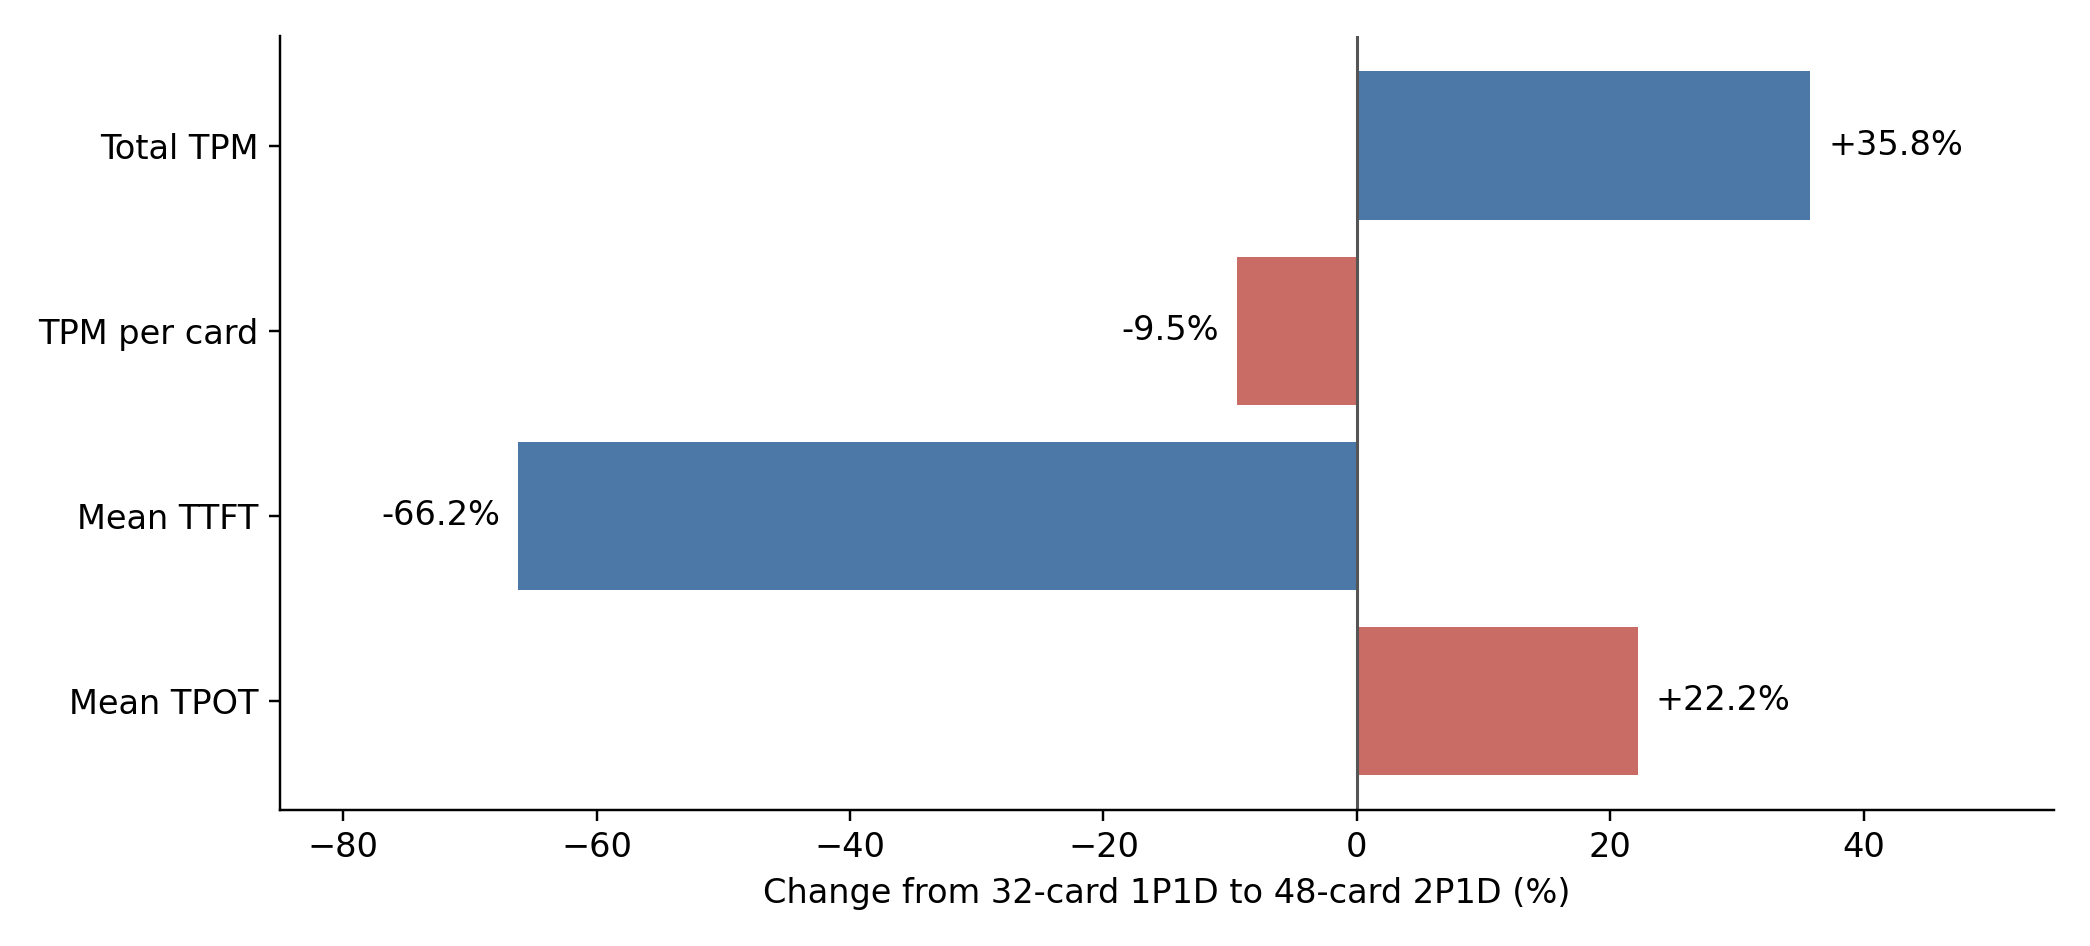
\includegraphics[width=\linewidth]{figures/resource_tradeoff.png}
\caption{96 并发下 32 卡 1P1D 与 48 卡 2P1D 的资源性能权衡。两次部署的机器组不同，变化率用于描述观测，不作为单因素效果。}
\label{fig:historical-resource}
\end{figure}

\subsection{故障诊断与执行状态}
重启实验暴露出运行时限制与部署状态之间的归因歧义。一次预填充参数调整后的失败最初提示运行时限制问题；后续测试又发现，已重启的预填充进程与常驻解码进程之间存在状态不兼容。之后的全量重启测试仍出现不稳定。这组观测说明，应在受控测试区分解释之前保留多个假设，不能由一次失败永久限制某个参数。

缓存加载实验进一步区分了进程存活与服务完成。在关闭异步加载的一次 1800 秒运行中，进程没有崩溃，但 14461 个请求仅有 992 个成功完成，成功率为 6.86\%。消除崩溃路径没有恢复有效服务，因此诊断还需检查调度进展、缓存加载、传输等待与请求完成。

24 小时会话重复测试在没有记录到进程崩溃的情况下，完成 284738 个请求中的 284733 个，完成率为 99.998244\%。另一次空闲 5.5 小时后的恢复测试发生故障，冷重启复测未复现该故障。持续运行与空闲恢复因此需要分别测试。这些现象提出了与状态有关的诊断问题，但尚不能确定恢复故障的唯一原因。

上述实验中的诊断干预由人工选择，skill 负责配置、资源会话准备、压测和报告。该流程为控制器提供可调用操作与既有经验。技能库编码干预条件和竞争解释，自主选择的价值则通过独立留出任务评价。

\section{问题定义}
\subsection{任务、配置与实际能力}
将任务定义为 $\tau=(m,w,h,v,\rho,\Delta,\mathcal{S})$。其中，$m$ 标识模型与固定精度，$w$ 为请求过程，$h$ 为拓扑，$v$ 为软件栈，$\rho$ 为初始化与状态协议，$\Delta$ 为评价时间范围，$\mathcal{S}$ 为服务目标。协议记录清缓存或复用、部署代次、空闲暴露、session 顺序和预热边界。这些属于控制条件，不代表假定内部状态均可观测。负载特征包括实际输入输出长度分布及到达波动。最大输出长度不能代替实测分布。

配置表示为
\begin{equation}
 c=(n_P,n_D,p_P,p_D,\pi,b_P,b_D,k),
\end{equation}
其中，$n_P,n_D$ 为副本数量，$p_P,p_D$ 为后端支持的并行策略，$\pi$ 为工作进程到资源的映射，$b_P,b_D$ 为运行时限制，$k$ 包含后端支持的状态传输设置。合法配置集合 $\mathcal{C}_{\tau}$ 由能力清单、显存可行性和资源可用性共同确定。同一比较中的模型与 KV 精度保持固定。这里的数量表示完整模型副本，而非任意切分模型权重所得的部分。

令 $A(c)$ 为分配的加速卡数量；当整机分配决定实际可回收资源时，另行记录节点数。本文不假定每个副本使用相同资源，也不假定某个模型能在特定数量的 P800 上运行。结构性配置变更可能需要重新部署。首版系统定位为离线规划器，不包含在线弹性伸缩或运行中请求迁移。

\subsection{服务可行性与优化目标}
对请求 $i$，定义
\begin{equation}
 z_i(c)=\mathbf{1}\{\text{complete}_i \land f_i\leq\theta_f
                  \land o_i\leq\theta_o\},
\end{equation}
其中，$f_i$ 为客户端观测的首 token 时延（TTFT），$o_i$ 为该请求输出 token 之间的平均间隔。主要负载至少包含两个输出 token；更短的完成请求将依据预先规定的适用性规则单独报告。失败、超时和被拒绝的请求仍计入提交请求总数这一分母。

对同一到达批次的 $N$ 个请求，联合达标率估计为
\begin{equation}
 \widehat a(c)=\frac{1}{N}\sum_{i=1}^{N}z_i(c).
\end{equation}
在稳定提交到达率 $\lambda$ 下，$\lambda\widehat a(c)$ 是达标请求到达率的估计。本文将其与按完成窗口统计的吞吐量区分，并报告请求到达、观测和队列排空区间。需要检查队列稳定性，并采用固定超时策略，防止较短测量窗口掩盖过载。各项时延分别满足边际尾部目标，并不意味着具有相同的联合达标率。

容量规划目标为
\begin{equation}
 \min_{c\in\mathcal{C}_{\tau}} A(c)
 \quad\text{满足}\quad
 a(c)\geq\alpha,\quad\text{队列稳定}.
 \label{eq:capacity}
\end{equation}
系统返回已找到的\emph{实测可行}配置中资源最少者，不给出全局最优保证。在相同资源层级内，次级目标为最大化达标服务能力。另设调优目标，最小化达到预先规定的可行性能目标所需成本。这些目标分别报告，不使用任意加权分数掩盖资源消耗与时延。

\subsection{预算约束下的证据获取}
在步骤 $t$，控制器从读取已有证据、执行诊断技能、评价配置及停止中选择动作 $a_t$。状态为 $s_t=(\tau,c_t,\mathcal{D}_t,\mathcal{K}_t,\mathcal{H}_t,B_t)$，包括观测、技能库、可修正的假设和剩余预算。$\mathcal{H}_t$ 不要求包含经过校准的概率。语言模型的自报置信度不是瓶颈概率的测量值。

每个动作均计入实际耗时 $T(a_t)$，以及资源成本
\begin{equation}
 C_A(a_t)=\int_{\text{动作区间}} A_t(u)\,du.
\end{equation}
诊断、模型加载、重启、预热、恢复及控制器推理均计入成本。并行实验需遵守统一资源上限，或使用相同的资源分配时长预算；所选口径必须在各方法之间保持一致。

\section{拟议方法}
\subsection{阶段感知证据，而非固定时延相加}
控制器使用阶段依赖图；在可以观测时，图中包括客户端提交、请求准入、预填充执行、状态就绪、状态传输、解码准入和 token 发出。该图描述具体部署的实现，不假定普遍适用的时延加和公式。传输与计算可能重叠。首个流式 token 的产生位置和转发路径取决于后端；未跟踪实际首 token 路径之前，不能直接将解码准入等待或 KV 传输时间计入 TTFT。

证据记录包括事件语义、时钟域、单位、样本量及缺失情况。跨节点时长需要使用已表征误差的同步时钟，或改为在单一时钟域内测量。语言模型接收记录引用和结构化摘要。不可用计数器标记为未知，不用看似合理的估计替代。诊断插桩开销单独测量，避免将其无声计入常规推理服务。

\subsection{将诊断技能表示为可执行实验}
定义技能为
\begin{equation}
 \sigma=(P,O,H,I,V,F,R,E,G),
\end{equation}
其中，$P$ 指定适用性，$O$ 为必要观测，$H$ 为解释集合，$I$ 为有边界的观测或干预，$V$ 将结果分为支持、反驳或无法判断，$F$ 为参数族，$R$ 为恢复流程，$E$ 为带来源的证据，$G$ 为外部检查的约束契约。初始技能由工程人员编写。既有干预用于初始化带上下文的假设与告警。

技能将诊断结果与调优收益分开。一项探测可能支持传输争用假设，但没有改善端到端有效吞吐；反过来，一个配置也可能改善目标，而其声称的原因仍未得到证实。两类观测不能自动互相验证。因此，记录中分别保存假设证据、服务可行性、资源使用和目标变化。

初始技能库拟覆盖预填充压力、解码容量或准入压力、PD 分配失衡，以及传输与计算相互影响。这些解释并非互斥，可能同时成立。每项技能必须说明固定什么、改变什么、是否需要重新部署，以及哪些情况会导致结果无法解释。缓存状态、精度、提交负载或总资源的临时变化，不能被包装成某个参数的孤立效应。

\subsection{历史经验约束下的技能执行}
拟议契约区分四类检查：
\begin{equation}
 G=(G_{\mathrm{cap}},G_{\mathrm{exec}},G_{\mathrm{eval}},G_{\mathrm{reuse}}).
\end{equation}
能力检查将操作限制在已部署的能力清单内；执行检查要求参数类型、资源预留、干预边界、恢复和预算限制；评价检查固定模型精度、负载协议、指标公式及 SLO 分母；复用检查将建议绑定到版本化状态上下文，必要时要求补充观测或重放。前置条件缺失时，返回明确的无法判断或不可执行结果，不能由语言模型暗中补齐。

\begin{table}[htbp]
\centering\small
\begin{tabularx}{\linewidth}{@{}>{\raggedright\arraybackslash}p{26mm}YY@{}}
\toprule
约束 & 执行条件 & 执行器行为 \\
\midrule
实际能力 & 后端支持的操作 & 拒绝能力清单外的操作 \\
执行与状态 & 重启状态一致性 & 核对进程代次，采用已声明恢复协议 \\
评价口径 & 进程与服务结果 & 分开记录存活、完成与联合 SLO 达标 \\
经验复用 & 执行上下文变化 & 重查缓存、空闲、软件与拓扑变化 \\
\bottomrule
\end{tabularx}
\caption{诊断技能执行的约束契约。}
\label{tab:contracts}
\end{table}

所有控制器共享相同的必要合法性与测量检查；固定规则基线获得相同技能和初始证据。否则，收益可能只是操作保障不一致，而非 Agent 决策。历史运行时参数告警只作为局部上下文建议；只有独立确认的能力约束才能硬性排除合法空间中的配置。

重启一致性说明了两者的区别：实验可对指定配置变更要求 P/D 协同重启，但经后端确认兼容的局部重启仍可按能力清单执行。不能由一次历史失败导出普遍重启规则。同样，关闭异步加载后不再崩溃，也不能直接认定调优成功，仍需单独测量服务可行性与成本。

每次调用记录约束判定、输入与上下文哈希、来源运行、预期可区分观测、结果、目标变化、恢复情况和全部成本。记录区分人工选择的干预与自主决策；后续反驳追加其范围和原因，同时保留原始观测。

\subsection{适用性检查与本地重放}
复用包含三层检查。首先，以可执行兼容性谓词检查技能所需的观测和动作。缺少必要能力时，拒绝该动作。若软件或模型变化的影响未知，则将技能在新上下文中标记为尚未验证；这不一定意味着诊断过程本身不合法。

其次，将当前上下文与证据记录中的上下文比较。负载与规模特征采用在源任务上固定的变换进行归一化，再用透明的距离与覆盖规则识别外推情况。阈值在源验证任务上选择，并在留出测试前固定。相似度只辅助检索，不保证结果正确。

最后，对过期、证据不足或超出覆盖范围的建议，执行其诊断动作的本地重放。重放可以重新支持预期、反驳预期，或仍然无法判断。无法判断不能算作负面结果。证据按任务和上下文保存，因此在某一拓扑下失效，不会抹去其他条件下仍成立的观测。重新验证减少缺乏支持的迁移，但不能普遍保证技能有用。

\subsection{诊断动作的选择}
语言模型提出数量受限的技能标识符列表，并附证据引用、竞争性解释及预期可区分观测。它输出结构化决策，不输出不受约束的脚本，也不能自行认定诊断成立。确定性检查器验证提案是否使用可用观测和合法干预。重复或不能区分现有解释的提案退回修改。

初始策略优先读取已收集证据，再选择预期能以较低成本区分未决解释的诊断。候选评分为
\begin{equation}
 Q(d)=\frac{U(d)}{\widehat C(d)+\varepsilon},
\end{equation}
其中，$U(d)$ 估计对当前解释的区分能力，$\widehat C(d)$ 估计所选统计口径下的成本。在获得经过校准的预测器之前，$U(d)$ 采用明确的工程等级评分，允许取“未知”；该分数表示等级，而非经过校准的信息增益或因果概率。评分规则、成本估计器及同分处理策略将在比较前固定。语言模型生成提案的价值，将与使用相同条件的固定规则选择器比较。

诊断证据更新得到支持、被反驳和仍未解决的预期集合。系统允许多个瓶颈同时存在。当现有探测不能区分解释时，控制器退回更广泛的数值探索。该退路很有必要：设计不假设每类负载都存在低成本且正确的诊断。

\subsection{不永久排除配置的数值搜索引导}
获得支持的诊断用于提高某个参数族的优先级，并建议合法初始化点。结构性提案包括副本数量和工作进程放置；在选定结构内部，数值优化器选择受支持的运行时参数。首版实现将使用一种明确记录的受约束优化器，并保留未经本文机制修改的版本作为基线。

除独立确定的能力约束之外，技能只影响提案优先级，不决定硬性可行性。具体而言，保留比例 $\epsilon>0$ 的提案机会用于完整合法空间：
\begin{equation}
 q_t(c)=(1-\epsilon)q_t^{\mathrm{guided}}(c)
                 +\epsilon q_t^{\mathrm{global}}(c).
\end{equation}
提案分布和 $\epsilon$ 的取值将在实现说明中给出。有限预算下，全局采样不能证明收敛；其目的是减少错误诊断带来的不可逆排除。固定的无改进规则可以触发重新诊断或增加全局探索，并记录额外成本。

最终接受的配置必须经过测量。预测器或 Agent 生成的解释，都不能使未测试配置成为最终推荐。最终评价冻结配置并使用独立请求，探索阶段的测量不能替代留出服务验证。

\subsection{证据更新与停止}
技能记录保留正面、负面和无法判断的结果、上下文特征、配置变化及原始运行标识。即使展示经验支持频率，也应说明它取决于已经执行的干预，不能解释为因果概率。控制器保留多个假设，不从稀疏运行中拟合不受约束的因果模型。

预算耗尽、达到预定目标并经过独立确认，或满足已声明终止规则时停止。Agent 可以提出停止请求，但由执行器检查规则。如果没有测得可行配置，输出应明确说明这一结果和已测试范围，不能暗中放宽 SLO 或更换模型。

\begin{figure}[t]
\centering
\resizebox{\linewidth}{!}{%
\begin{tikzpicture}[node distance=7mm and 9mm,box/.style={draw=black!55,rounded corners,align=center,font=\small,text width=39mm,minimum height=13mm},arr/.style={-{Latex[length=2mm]},thick}]
\node[box] (state) {任务、能力清单\\与观测};
\node[box,right=of state] (agent) {Agent 提出\\诊断技能提案};
\node[box,right=of agent] (gate) {检查技能约束\\必要时重放};
\node[box,below=of gate] (probe) {执行诊断\\记录证据};
\node[box,left=of probe] (search) {调整参数族优先级\\执行数值搜索};
\node[box,left=of search] (eval) {独立评价\\冻结推荐配置};
\draw[arr] (state)--(agent); \draw[arr] (agent)--(gate);
\draw[arr] (gate)--(probe); \draw[arr] (probe)--(search);
\draw[arr] (search)--(eval); \draw[arr] (eval)--(state);
\end{tikzpicture}%
}
\caption{诊断技能框架的控制流程，证据更新保留对应干预的来源。}
\label{fig:architecture}
\end{figure}

\section{系统设计与算法}
\subsection{SGLang 与 P800 的适配边界}
适配器拟提供能力发现、部署、观测收集、诊断执行、压测执行、恢复及配置冻结。逻辑参数先经部署版本检查，再转换为具体启动参数。控制器运行在 token 生成热路径之外，不作为逐 token 调度器。

能力清单记录模型与分词器标识、权重与 KV 类型、运行时与插件修订版本、注意力实现、并行配置、图执行与缓存模式、传输后端，以及支持的路由方式。实际盘点 CPU、XPU、PCIe 和网卡拓扑，不能从 CPU 插槽数推断。能力发现记录当前部署的设备显存、网络接口与传输行为。

部署操作同时包含资源预留和恢复方案。诊断探测在指定实验资源上运行，所有压测解析和目标计算都在 Agent 可编辑决策之外完成。Agent 只能选择已注册操作，不能在比较过程中修改评价输入、指标公式或基线配置。评价器与控制器保持独立。

\Needspace{8\baselineskip}
\subsection{拟议算法}
\begin{quote}\small
\textbf{输入：}任务、合法资源、能力清单、初始技能库与预算。\\
1. 测量预先声明的初始配置，创建证据记录。\\
2. 在预算尚未耗尽时循环：\\
\hspace*{1em}a. 检索兼容的候选技能及上下文记录。\\
\hspace*{1em}b. 请求控制器输出结构化诊断提案。\\
\hspace*{1em}c. 检查约束和状态，读取证据或重放诊断。\\
\hspace*{1em}d. 记录证据、来源和服务结果。\\
\hspace*{1em}e. 通过引导搜索与全局搜索提出合法配置。\\
\hspace*{1em}f. 部署、预热、测量，必要时恢复；计算全部成本。\\
\hspace*{1em}g. 更新优化器及对应上下文的技能记录。\\
\hspace*{1em}h. 检查预先声明的停止或重新诊断规则。\\
3. 冻结已测得的最佳可行候选，并进行独立验证。\\
\textbf{输出：}配置与证据；或报告未测得可行配置。
\end{quote}
该算法定义拟议自主循环，在已有 skill 执行流程上区分诊断选择、配置搜索与独立评价。

\section{评价方法}
\subsection{研究问题}
RQ1：相较受约束数值搜索和普通工具型 Agent，本文方法能否更快达到预定可行目标？RQ2：相较拥有相同技能的固定规则控制器，诊断选择是否改变了有效的配置决策？RQ3：本地重放与适用性检查是否改善技能向留出上下文的迁移？RQ4：在不同部署规模下，最终推荐的资源消耗与达标服务能力表现如何？

\subsection{环境、任务与数据划分}
评价使用第~\ref{sec:historical} 节的 P800 资源池，同一比较固定模型 checkpoint 与精度。在完整副本为 16 卡且路由受支持的条件下，计划比较 48 卡的 2P1D/1P2D 与 64 卡的 3P1D/2P2D/1P3D，并保留 32 卡 1P1D。每种布局先通过能力与显存检查。后端支持时，以第二种模型配置评价泛化。

负载覆盖短输入短输出、长输入短输出、短输入长输出及混合长度。开环到达用于评价服务容量与队列稳定性，固定并发用于补充压力和机制测试。冷态初始化、重复复用及空闲恢复分别评价。

开发实验用于编写初始技能，其上下文变换和阈值在源验证任务上选择，再冻结后用于留出的模型、负载、状态或规模任务。分别报告冷启动调优、带历史经验调优和任务内更新。所有控制器具有相同初始知识、合法操作、资源上限及成本核算口径。

\subsection{基线与组件归因}
\begin{table}[H]
\centering\small
\begin{tabularx}{\linewidth}{@{}>{\raggedright\arraybackslash}p{30mm}YY@{}}
\toprule
方法 & 共同条件 & 比较目的 \\
\midrule
已调优原生服务 & 同置或分块预填充及原生 PD；固定模型和精度 & 端到端工程参照 \\
受约束优化器 & 相同合法空间、预算及测量流程 & 检验超出数值搜索的收益 \\
固定规则控制器 & 相同技能、观测与初始知识 & 检验语言模型决策的必要性 \\
工具型 Agent & 相同模型与工具；普通反馈和日志检索 & 检验超出通用 Agent 编排的收益 \\
无条件技能复用 & 同库；保留必要检查，不重验历史建议 & 检验错误迁移的代价 \\
完整方案 & 包含全部已声明组件 & 检验联合效果及开销 \\
\bottomrule
\end{tabularx}
\caption{控制器对照及共同评价条件。}
\end{table}

知识积累 Agent 基线参考 STELLAR 与 SysInsight，适配 SGLang 时使用相同证据和执行接口，以本地测量结果进行比较。消融实验将分别移除主动诊断、以原始日志检索替换技能记录、禁用适用性重放，以及移除全局探索，每次只改变一个机制。

\subsection{指标、不确定性与资源核算}
主要指标包括达到预定目标所需的资源分配时长与实际耗时、联合 SLO 达标率，以及相同提交负载下最终实测资源占用。次要指标包括输出 token 吞吐、实际输入输出长度、请求级 TTFT 与 TPOT、token 级相邻 token 时延、失败配置、重新部署和诊断动作。P99 结果需要充分样本量和明确的不确定性。只有在解释受控或经独立确认的场景，才报告诊断准确率。

计划对核心服务配置点至少进行三次独立重复；控制器与搜索使用多个随机种子，在预算允许时初始设置为五个。运行顺序随机化或交错安排，配对比较使用相同的负载实现。一次过载运行中的请求，不能视为整个调优过程的独立重复。未达到目标的运行作为删失结果报告，不能在计算达标耗时时将其丢弃。

最终评价前固定阈值、模型选择、搜索范围、停止条件、Agent 提示词、生成设置和 token 预算。Agent 推理使用独立容量，或明确测量其造成的干扰。并行搜索共享相同资源上限，或按相同资源分配时长预算比较。离线建库与后续调优成本分别报告；经验复用的摊销收益需要计算，不能直接假定。

\subsection{机制测试与决策后果}
若后端暴露适当操作，首项机制测试比较独立传输、独立解码及二者受控并发执行。另一项比较阶段容量估计给出的推荐与端到端配置排名。这些测试用于检验阶段估计能否区分端到端配置选择。

对每次成功诊断，追踪完整决策链：已有观测、考虑的备选解释、所选探测、探测结果、搜索优先级变化、最终配置及独立验证。对错误诊断，报告浪费成本，以及重放或全局探索是否帮助恢复。该分析将技能机制与可测结果连接起来，避免将解释质量当作性能收益的替代指标。



\section{局限与有效性威胁}
部署实验覆盖一个加速卡系列和一类会话负载。部分比较同时改变机器组、执行时长、缓存状态或实际输出长度，因此用于形成假设，不能隔离唯一机制。汇总时延不能建立尾时延或联合 SLO 达标结果，这些测量需要请求级 trace 和独立重复运行。

拟议 Agent 控制器尚未完成同条件自主调优实验。当前观测来自人工选择干预与 skill 执行，支撑技能设计，但没有建立相对数值优化、固定规则或既有调优 Agent 的优势。评价方法分别检验这些贡献，并计入诊断与恢复开销。

可观测性与插桩也影响有效性。阶段事件缺失可能使竞争解释无法区分，插桩本身可能扰动执行；缓存特征与阈值可能对开发任务过拟合。即使只改变一个配置字段，网络波动、共享资源和输出长度变化仍可能混淆干预结果。

语言模型可能遗漏解释或误解参数语义。注册动作、显式证据和独立检查可降低风险，但不保证诊断正确。调优耗时减少与最终服务能力改善是两个不同结果。本文范围不包括自动算子重写、精度与质量权衡、跨厂商 KV 互操作或生产在线迁移。

\section{结论}
本文提出面向 SGLang PD 服务的经验约束诊断技能与 Agent 自动调优框架。P800 部署实验引出三项需求：将执行状态与性能共同记录，区分进程存活和有效服务，以及联合评价资源效率与时延。框架将这些需求落实为有边界的干预、上下文相关复用和受约束数值搜索。核心研究问题是，选择并重验诊断动作能否降低找到可行配置的完整成本。同条件自主控制器评价仍是后续工作。



{\footnotesize
\interlinepenalty=10000
\setlength{\bibsep}{2pt plus 1pt minus 1pt}
\bibliographystyle{elsarticle-num}
\bibliography{references}
}
\end{document}
